\newpage
\section{Pianificazione}
Per migliorare lo sviluppo del progetto, il team ha deciso di suddividere il carico di lavoro in sei periodi:
\begin{itemize}
	\item \textbf{Analisi dei Requisiti (AR)};
	\item \textbf{Analisi dei Requisiti in dettaglio (AD)};
	\item \textbf{Progettazione architetturale (PA)};
	\item \textbf{Progettazione di dettaglio (PD)};
	\item \textbf{Codifica (CO)};
	\item \textbf{Verifica e Validazione (VV)}.
\end{itemize}

Per evidenziare le attività principali di un periodo, ad ognuno di essi viene associato un diagramma di \textit{Gantt\ped{G}}. 
Ogni attività, a propria volta, può essere suddivisa in sotto-attività e fare riferimento ad una o più risorse.
Una \textit{milestone\ped{G}} può essere esterna, coincidendo con le date di consegna dei documenti o con l'approvazione del lavoro svolto fino a quel moneto, o interna, ovvero un punto di revisione stabilito dal team. 
La rappresentazione temporale di queste nel diagramma di \textit{Gantt\ped{G}} avviene mediante linee nere le cui estremità sono delle frecce verso il basso. 
Oppure con dei rombi neri nel caso in cui la finestra di tempo che rappresentano sia di piccola durata. 
Le attività corrispondono a delle \textit{milestone\ped{G}} interne. 
Il momento in cui un periodo termina coincide con una \textit{milestone\ped{G}}.\\
I diagrammi di \textit{Gantt\ped{G}} permettono, grazie all'uso di frecce, di rappresentare le dipendenze tra le attività.
La conseguenza di un ritardo su un'attività è lo slittamento temporale di tutte le attività ad essa correlate . \\
Si è deciso di non riportare i diagrammi di \textit{PERT\ped{G}} in quanto poco leggibili data la moltitudine
di nodi presenti; quindi si è scelto di presentare i soli diagrammi di \textit{Gantt\ped{G}} riportando anche le
risorse impegnate per ciascuna attività.




\subsection{Suddivisione delle attività}
\subsubsection{Analisi dei Requisiti}
\textbf{Periodo:} dall'8 Dicembre 2015 al 22 Gennaio 2016.
Questo perdiodo inizia in concomitanza alla formazione del gruppo e termina con la consegna dei documenti per la \textbf{Revisione dei Requisiti}.
\begin{itemize}
		\item \textbf{Norme di Progetto}: questo è il primo documento redatto in ordine cronologico poiché norma tutto l'operato del team rigaurdo la stesura dei documenti, delle comunicazioni, etc. ed è indipendente dal capitolato scelto. E' l’Amministratore di Progetto a redigere questo documento inserendovi le norme che il team dovrà seguire durante lo svolgimento di tutte le attività. Verificatori certificheranno che tutte le norme siano state effettivamente osservate durante le diverse attività;
		\item \textbf{Studio di Fattibilità}: in questo documento vengono analizzati tutti i capitolati proposti. Per ognuno viene analizzato il dominio tecnologico e applicativo valutandone i fattori positivi e negativi. Risulta essere un attività	critica perché definisce il progetto sul quale il gruppo andrà a lavorare e blocca la stesura del documento di Analisi dei Requisiti;
		\item \textbf{Analisi dei Requisiti}: redatto dagli Analisti, è l'analisi approfondita del capitolato scelto con lo Studio di Fattibilità;
		\item \textbf{Piano di Progetto}: redatto dal Responsabile di Progetto, individua tutte le attività necessarie alla conclusione del progetto e le assegna alle risorse disponibili distribuendo il carico di lavoro in maniera uniforme;
		\item \textbf{Piano di Qualifica}: steso dal Verificatore, definisce come devono essere effettuate le verifiche al fine di consegnare un prodotto di qualità;
		\item \textbf{Glossario}: scritto in maniera incrementale dai redattori dei diversi documenti e contiene la spiegazione di alcuni termini utilizzati nei vari documenti, al fine di eliminare ogni possibile	ambiguità di significato;
		\item \textbf{Lettera di presentazione}: documento che dichiara l’interesse del gruppo a partecipare alla gara d’appalto.
\end{itemize}
In questa fase i ruoli maggiormente interessati sono quelli di Amministratore, Responsabile, Analista e Verificatore. 

\begin{sidewaysfigure}
	\centering
	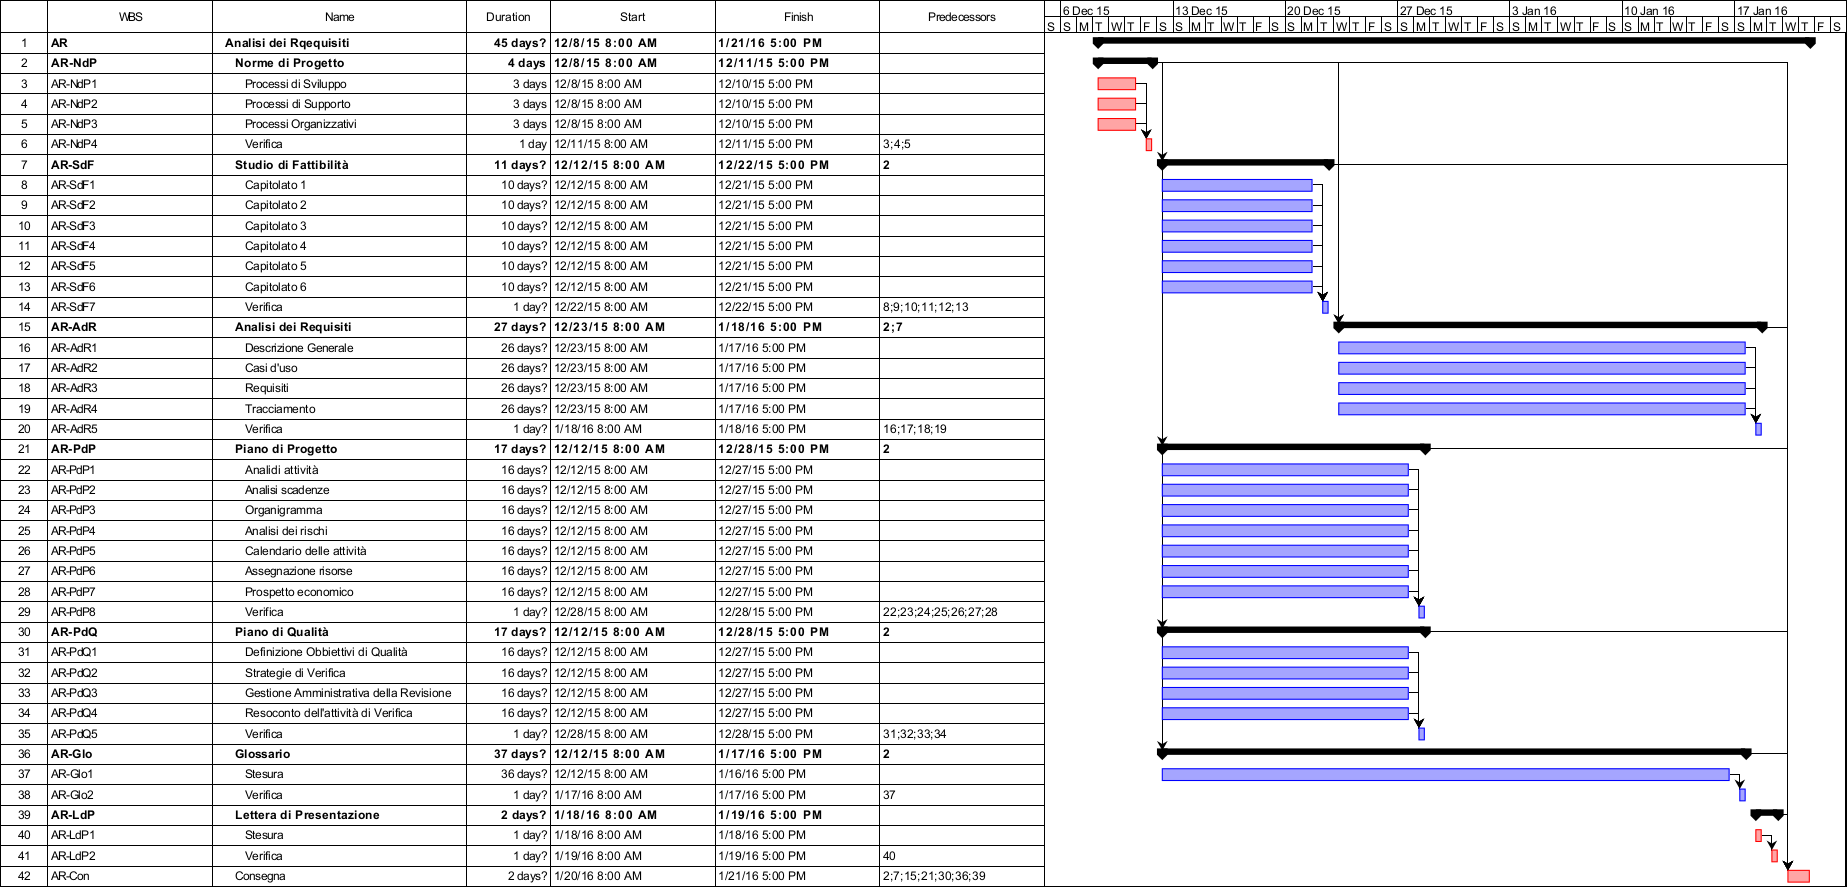
\includegraphics[keepaspectratio = true, width=24cm]{immagini/PdP_AnalisiDeiRequisitiGantt.png}
	\caption{Diagramma di Gantt relativo al periodo di Analisi dei Requisiti.}\label{etichetta}
\end{sidewaysfigure}
\newpage
\subsubsection{Analisi dei Requisiti in Dettaglio}
\textbf{Periodo:} dal 17 Febbraio 2016 al 22 Febbraio 2016. 
\subsubsection{Progettazione Architetturale}
\textbf{Periodo:} dal 23 Marzo 2016 al 20 Marzo 2016. 
\subsubsection{Progettazione di Dettaglio}
\textbf{Periodo:} dal 21 Marzo all'11 Aprile 2016.
\subsubsection{Codifica}
\textbf{Periodo:} dal 19 Aprile 2015 al 16 Maggio 2015. 
\subsubsection{Verifica e Validazione}
\textbf{Periodo:} dal 24 Maggio 2016 al 10 Giugno 2016. 